\documentclass{standalone}
\usepackage{amsmath}
\usepackage{tikz}
\usetikzlibrary{automata, positioning}

\begin{document}

    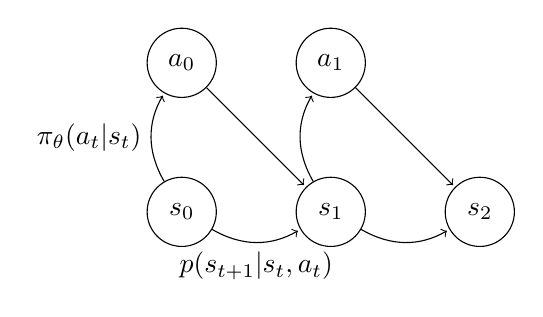
\begin{tikzpicture}
        % Add the states
        \node[state]             (s0) {$s_0$};
        \node[state, right=of s0] (s1) {$s_1$};
        \node[state, right=of s1] (s2) {$s_2$};
        \node[state, above=of s0] (a0) {$a_0$};
        \node[state, above=of s1] (a1) {$a_1$};

        \draw[every loop]
            (s0) edge[bend right, auto=right] node {$p(s_{t+1}\vert s_t, a_t)$} (s1)
            (s0) edge[bend left, auto=left] node {$\pi_\theta(a_t \vert s_t)$} (a0)
            (s1) edge[bend right] node {} (s2)
            (s1) edge[bend left] node {} (a1)
            (a0) edge[] node {} (s1)
            (a1) edge[] node {} (s2);
    \end{tikzpicture}

\end{document}
